\section{Data reduktion}

\begin{frame}{Identificer partikler}
	\begin{itemize}
		\onslide<2->{\item Forskellige energi afsætning} 
		\onslide<3->{\item \al-partikler bliver stoppet af \SI{60}{\mu m}} 
		\onslide<4->{\item \be-partikler afsætter \SI{300}{keV} - \SI{500}{keV} pr. mm silicium} 
		\onslide<5->{\item Overlappende energi} 
		\onslide<6->{\item \be-partikler bliver opfanget af PAD} 
	\end{itemize}
\end{frame}

%\begin{frame}{Identificer partikler}
%	\begin{itemize}
%		\onslide<2->{\item Alle hits kan være mulige \al-partikler} 
%		\onslide<3->{\item Hvis et hit rammer PAD $\rightarrow$ \be-partikel} 
%		\onslide<4->{\item Hvis et hit rammer Det2 eller DetD $\rightarrow$ mulig \be-partikel} 
%		\onslide<5->{\item Flere end 2 partikler $\rightarrow$ lavest indbyrdes impuls er \al-\al\ par} 
%	\end{itemize}
%\end{frame}

\begin{frame}{Vinkel cut}
	Grundet impuls bevarelse, forventer vi $180 \degree $ mellem \al-partiklerne\\
	Langt største delen af hits i eksperimentet har tæt på $180 \degree$ mellem sig\\
	Vi vælger $\cos(\theta) \leq -0.95$\\
	Svare til $161\degree$
	\begin{figure}
		\centering
		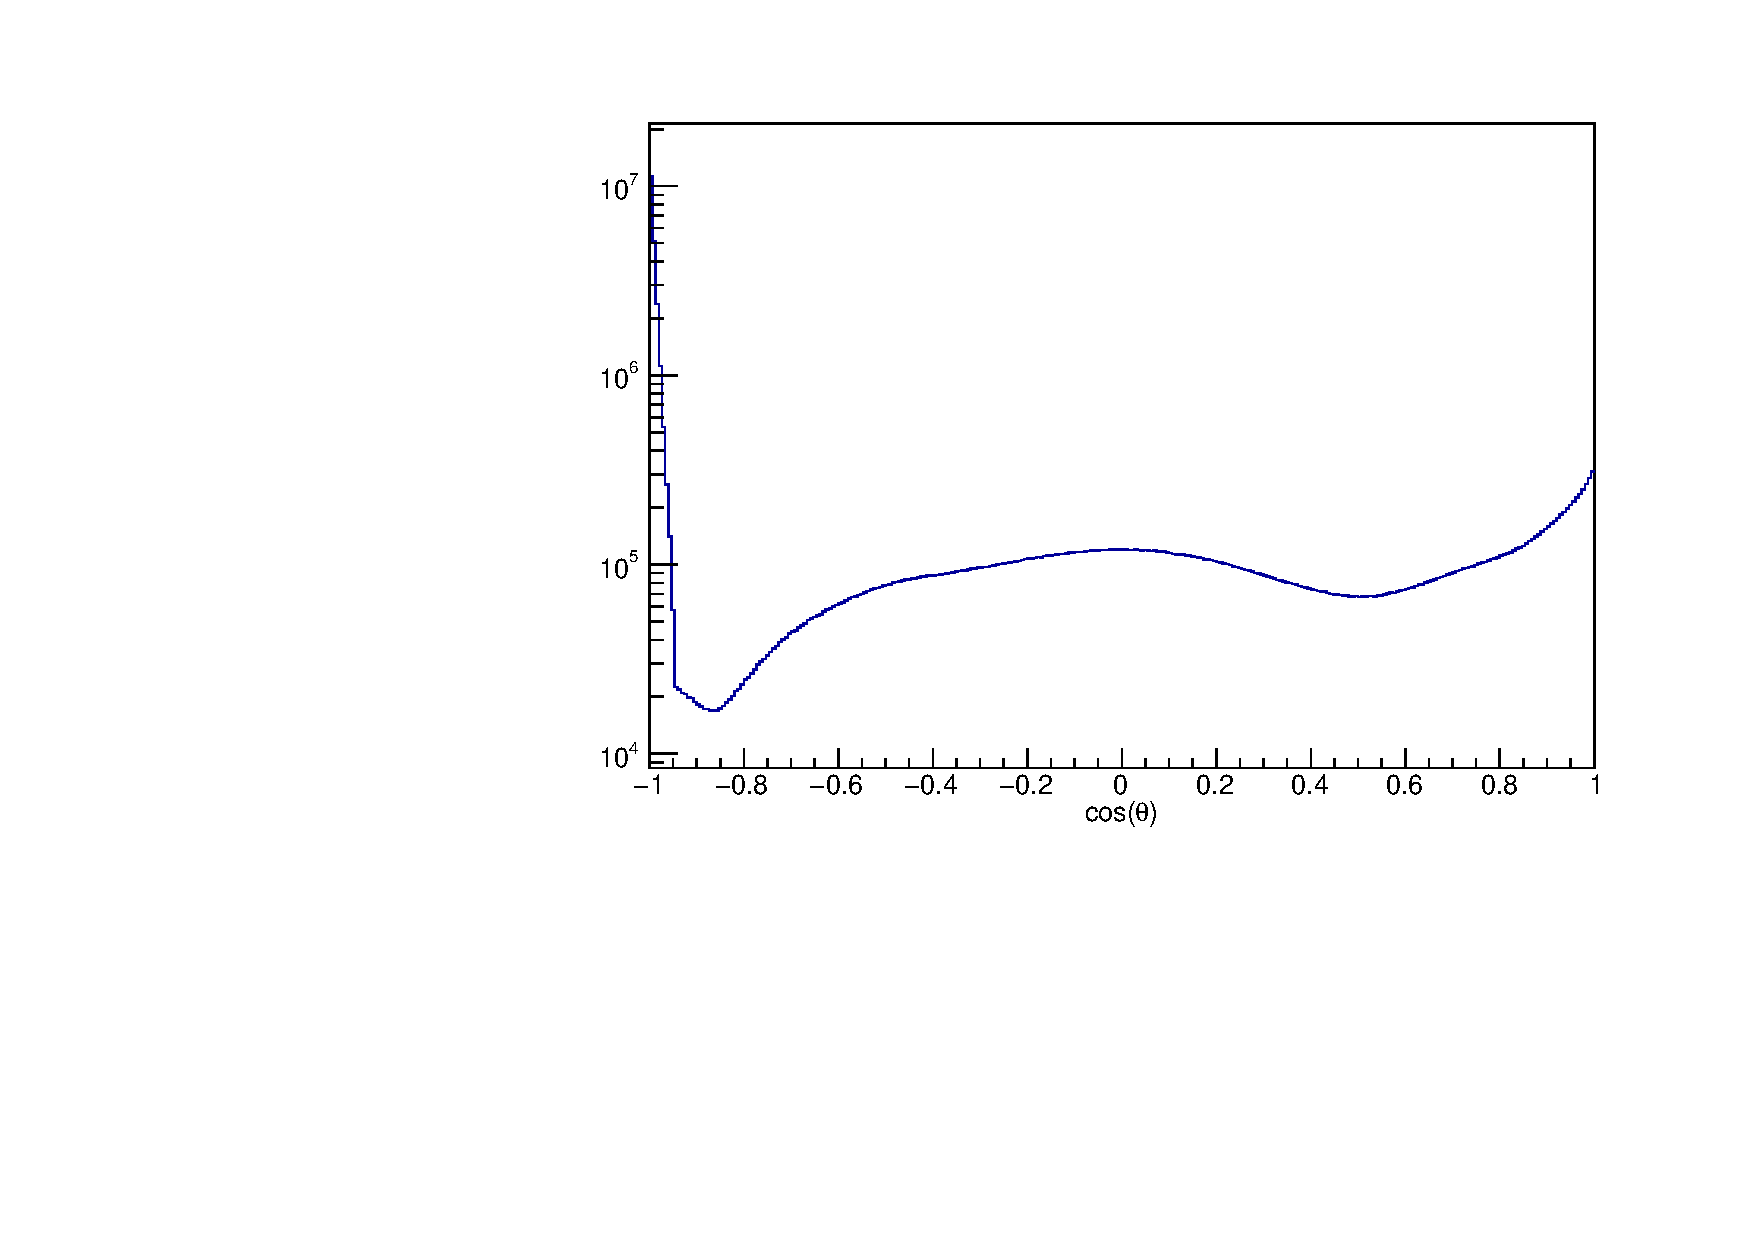
\includegraphics[width=.7\columnwidth]{../figures/cosang.pdf}
	\end{figure}
\end{frame}

\begin{frame}{Impuls cut}
	Enkelt \al-partikel med \SI{1.5}{MeV} har impuls på \SI{105}{MeV/c}\\
	Enkelt \be-partikel med \SI{3}{MeV} har impuls på \SI{1.7}{MeV/c}\\
	Størrelsen af den samlede impuls må maksimalt være \SI{40}{MeV/c}
	\begin{figure}
		\centering
		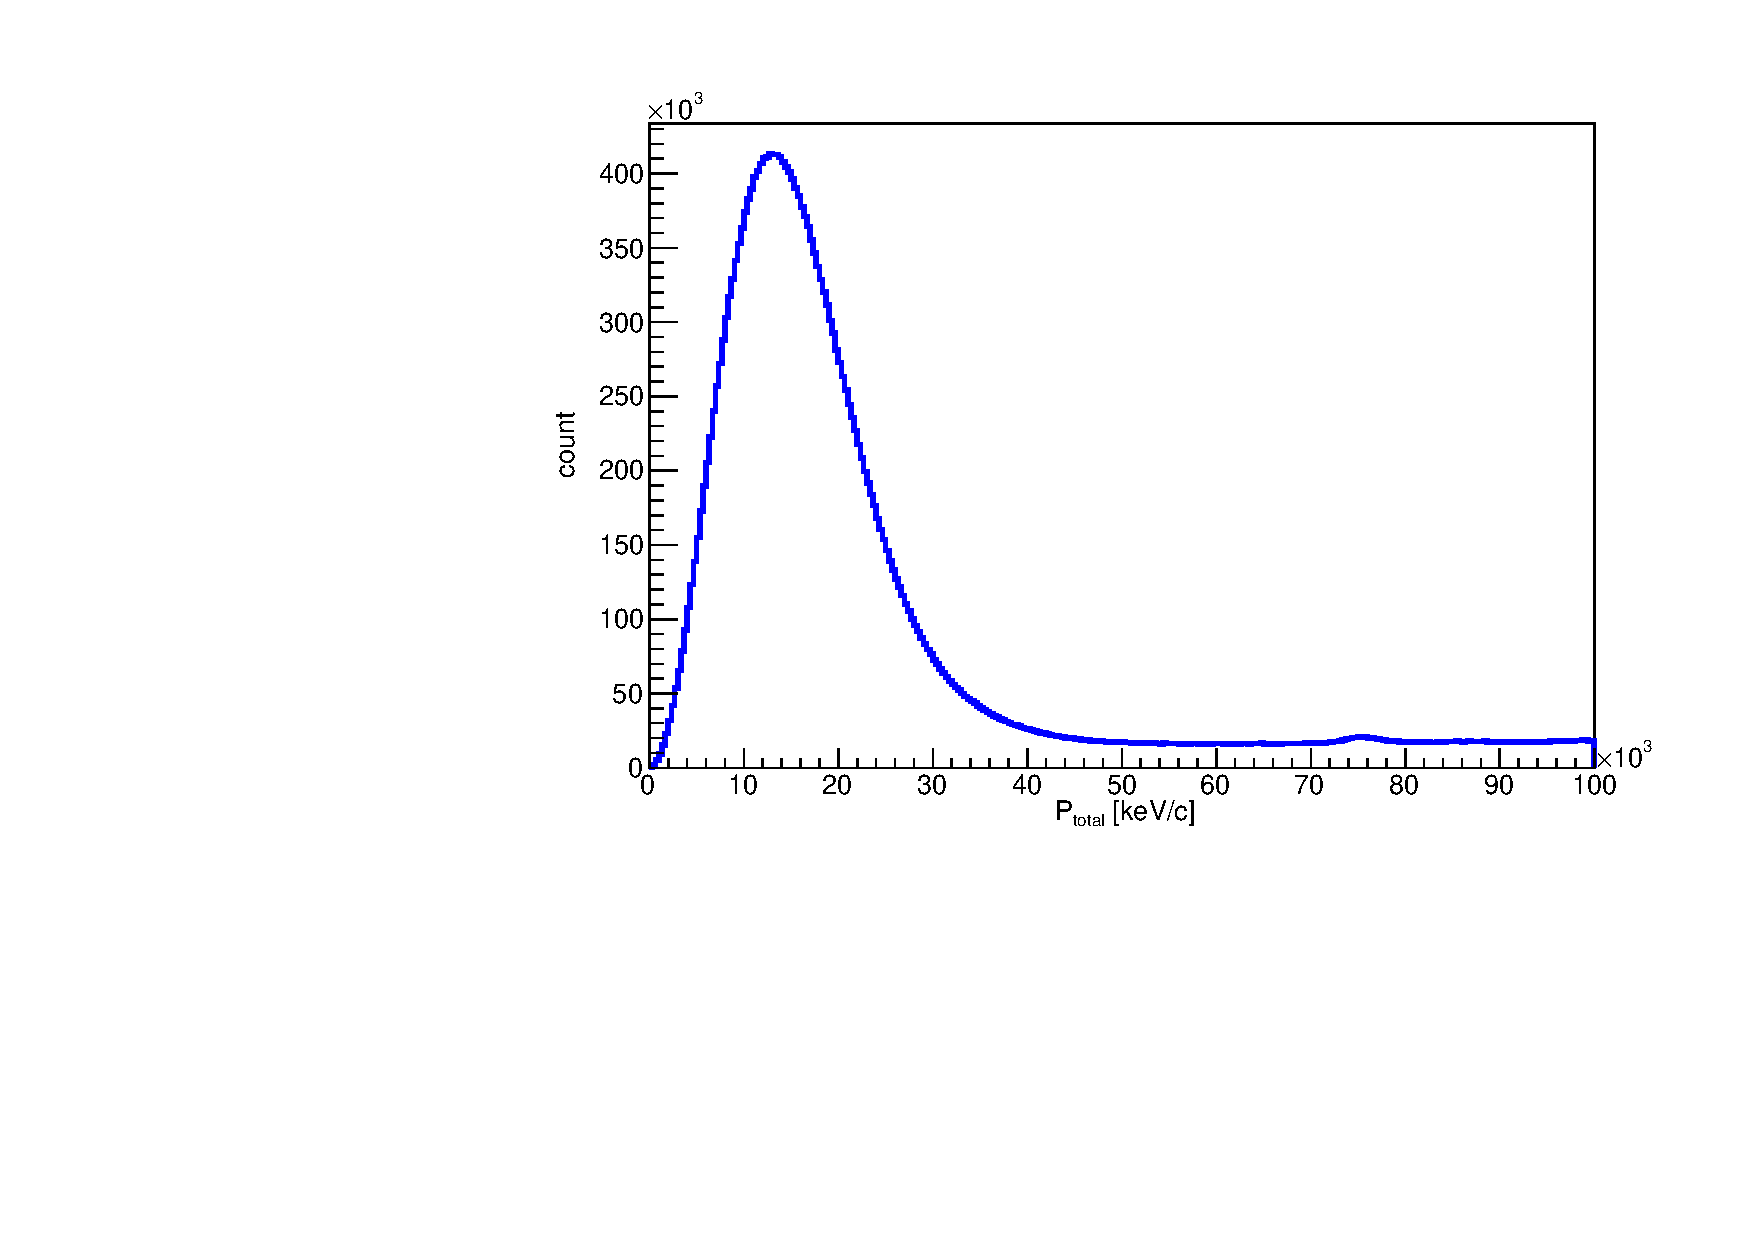
\includegraphics[width=.7\columnwidth]{../figures/ptotNoCut.pdf}
	\end{figure}
\end{frame}

\begin{frame}{\be\ multiplicitet cut}
	Kræver mindst én \be-partiel\\
	Flere \be-partikler kan skyldes spredning af enkelt \be\\
	Isotrop vinkelfordeling $\rightarrow$ antal irrelevant
	\begin{figure}
		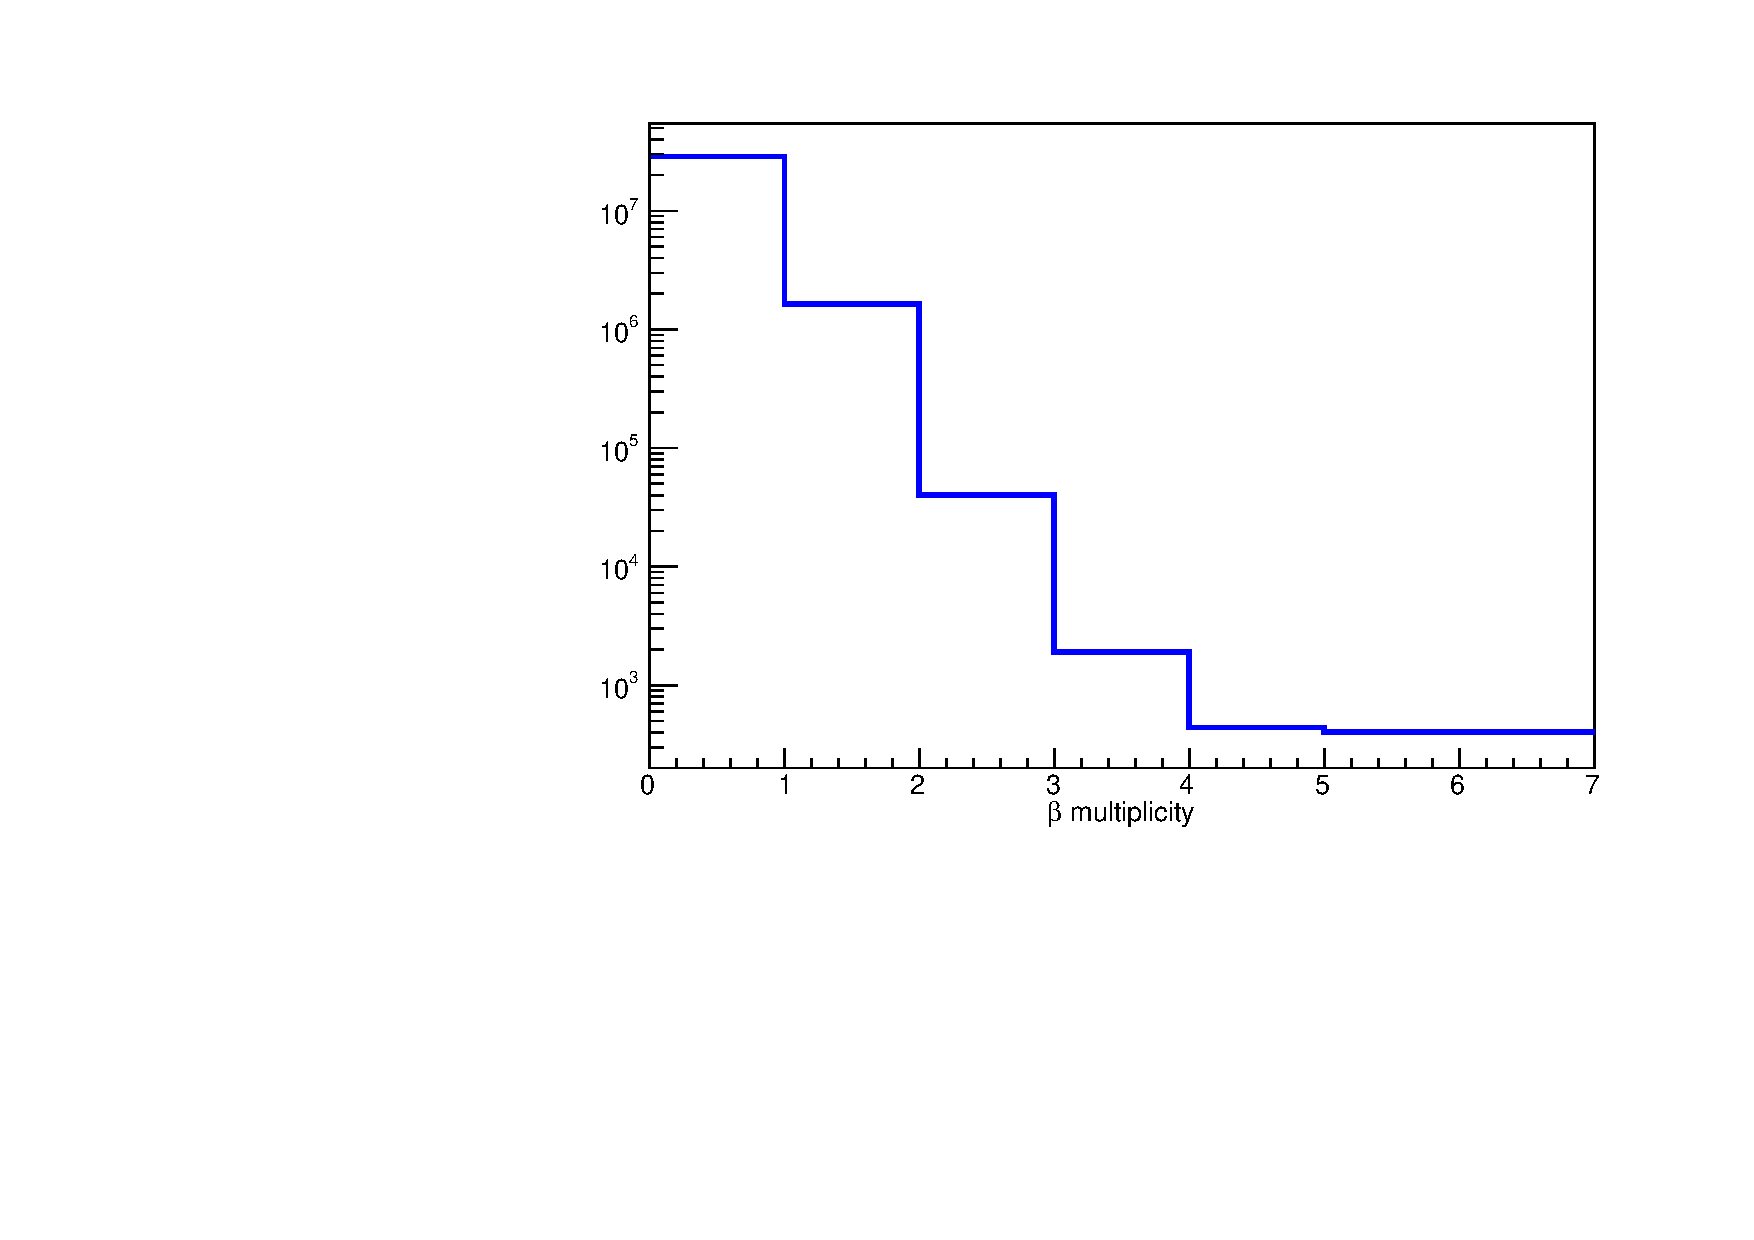
\includegraphics[width=.7\columnwidth]{../figures/betaMul.pdf}
	\end{figure}
\end{frame}
